%%%%%%%%%%%%%%%%%%%%%%%%%%%%%%%%%%%%%%%%%
% Journal Article
% LaTeX Template
% Version 1.4 (15/5/16)
%
% This template has been downloaded from:
% http://www.LaTeXTemplates.com
%
% Original author:
% Frits Wenneker (http://www.howtotex.com) with extensive modifications by
% Vel (vel@LaTeXTemplates.com)
%
% License:
% CC BY-NC-SA 3.0 (http://creativecommons.org/licenses/by-nc-sa/3.0/)
%
%%%%%%%%%%%%%%%%%%%%%%%%%%%%%%%%%%%%%%%%%

%----------------------------------------------------------------------------------------
%	PACKAGES AND OTHER DOCUMENT CONFIGURATIONS
%----------------------------------------------------------------------------------------

\documentclass[twoside,twocolumn,paper=letter,fontsize=11pt]{article}
\usepackage[cm]{fullpage} 

\usepackage{blindtext} % Package to generate dummy text throughout this template 

\usepackage[sc]{mathpazo} % Use the Palatino font
\usepackage[T1]{fontenc} % Use 8-bit encoding that has 256 glyphs
\linespread{1.05} % Line spacing - Palatino needs more space between lines
\setlength\parindent{0pt}
\usepackage[protrusion=true,expansion=true]{microtype} % Slightly tweak font spacing for aesthetics

\usepackage[english]{babel} % Language hyphenation and typographical rules

%\usepackage[hmarginratio=1:1,top=32mm,columnsep=20pt]{geometry} % Document margins
\usepackage[hang, small,labelfont=bf,up,textfont=it,up]{caption} % Custom captions under/above floats in tables or figures
\usepackage{booktabs} % Horizontal rules in tables

\usepackage{lettrine} % The lettrine is the first enlarged letter at the beginning of the text
\usepackage{multirow}

\usepackage{enumitem} % Customized lists
\setlist[itemize]{noitemsep} % Make itemize lists more compact

\usepackage{abstract} % Allows abstract customization
\renewcommand{\abstractnamefont}{\normalfont\bfseries} % Set the "Abstract" text to bold
\renewcommand{\abstracttextfont}{\normalfont\small\itshape} % Set the abstract itself to small italic text

\usepackage{titlesec} % Allows customization of titles
\renewcommand\thesection{\Roman{section}} % Roman numerals for the sections
\renewcommand\thesubsection{\roman{subsection}} % roman numerals for subsections
\titleformat{\section}[block]{\large\scshape\centering}{\thesection.}{1em}{} % Change the look of the section titles
\titleformat{\subsection}[block]{\large}{\thesubsection.}{1em}{} % Change the look of the section titles

\usepackage{fancyhdr} % Headers and footers
\pagestyle{fancy} % All pages have headers and footers
\fancyhead{} % Blank out the default header
\fancyfoot{} % Blank out the default footer
%\fancyhead[C]{Running title $\bullet$ May 2016 $\bullet$ Vol. XXI, No. 1} % Custom header text
\fancyfoot[RO,LE]{\thepage} % Custom footer text

\usepackage{titling} % Customizing the title section

\usepackage{hyperref} % For hyperlinks in the PDF
\usepackage{graphicx} % Including graphics
\usepackage{subcaption} % Including subfigures
\usepackage{stfloats} 
%----------------------------------------------------------------------------------------
%	TITLE SECTION
%----------------------------------------------------------------------------------------

\setlength{\droptitle}{-4\baselineskip} % Move the title up

\pretitle{\begin{center}\Large\bfseries} % Article title formatting
\posttitle{\end{center}} % Article title closing formatting
\title{Applying Machine Learning to Predict and Explain Primate Consortship} % Article title
\author{%
\textsc{Josh King} \\[1ex] 
\and 
\textsc{Vayu Kishore} \\[1ex] 
\and 
\textsc{Filippo Ranalli} \\[1ex] 
}
\date{} % Leave empty to omit a date
\renewcommand{\maketitlehookd}{%
%\begin{abstract}
%\noindent \blindtext % Dummy abstract text - replace \blindtext with your abstract text
%\end{abstract}
}

%----------------------------------------------------------------------------------------

\begin{document}

% Print the title
\maketitle
%----------------------------------------------------------------------------------------
%	ARTICLE CONTENTS
%----------------------------------------------------------------------------------------

\section{Introduction}

% \lettrine[nindent=0em,lines=3]{T} \\

\lettrine[nindent=0em,lines=3]{W}e apply machine learning methods to
investigate the behavioral and genetic reasons for success and failure of mating
between wild baboon pairs. The mating behavior of a species drives genetic
interchange and is a major driver of evolution within populations. Factors that
contribute to consortship may range from genetic causes, such as physical traits
expressed due to the presence of a gene, to those that are social or behavioral.
The contribution of social factors is of particular interest for animals that
live in structured groups, where factors such as rank within a social heirarchy
may impact mating success.  Investigating this topic will provide deeper insight
into the factors of mating success in social mammals, which may be extended to
apply to humans as well.\\

Our analysis applies machine learning methods to examine whether successful
consortships can be predicted, and whether certain behavioral or genetic
features are especially relevant in determining consortship. More specifically,
our input is a set of interactions between wild male and female baboons, where
the features are various attributes of the pair and the label is whether
consortship occurred. We try to predict successful consortships by classifying
by using SVM, AdaBoosting, Random Forest, and graphical edge prediction.
Moreover, we apply graphical algorithms to try to capture latent features and
test whether they improve our classification accuracy.  Additionally, we apply
k-means to see whether successful and unsuccessful pairs can be clustered.

%------------------------------------------------

\section{Related Work}

\cite{Tung:2012} examine the impact of behavioral and genetic effects on
consortship in male/female baboon pairs in a wild yellow baboon population. They
found that a mix of both genetic and social factors drive non-random mating
within populations.

\section{Dataset and Features}
\subsection{Description}
The dataset that we use was collected and analyzed using statistical methods by
\cite{Tung:2012}. It contains observations about the success of potential
baboon mating pairs. In particular, it specifies if , male/female baboon
pairings were successful in consorting when given the opportunity.  There are
approximately 12,000 observations of interactions between 115 females and 121
males, with 1648 instances of consortship, and the features are a mix of
behavioral data such as the rank difference between the male and female pair,
as well as genetic data, such as the estimated genetic distance between the
pair. 

There are several categories of features present within the dataset.
\begin{itemize}
  \item{\textbf{Observed biological and genetic features}: These include female age
    and conceptiveness, as well as the estimated genetic diversity and genetic
    distance between the mating pair.}
  \item{\textbf{Observed behavioral features}: These include rank of the mating pair
    within the social heirarchy of the group and how many males and females from
    their group were present when the interaction of the pair took place.}
  \item{\textbf{Derived Pairwise Features}: Some features are
    transformations applied to the observed features described above, which were
    computed by \cite{Tung:2012}. Some of the transformations compute a pairwise
    score based on a combination of the male and female attributes. For example,
    the rank\_interact feature represents the combination of male and female
    ranks and the assort\_index uses genetic distance between the pair to
    calculate a measure of inbreeding avoidance.
    }
  \item{\textbf{Derived Single Features}: The remaining features are single
    raw features which are scaled based on an assumed distribution.  The
    male\_rank\_transform feature, for example, scales the male rank based on an
    exponential distribution.}
\end{itemize}

In addition to the different categories, some of the features, such as
(untransformed) rank, are ordinal, while others, such as estimated genetic
distance are real-valued.\\

% \subsection{Identifiers and Labels}
Each datapoint contains an identifier of the male and female pair in an
interaction that could lead to a consortship and a 0/1 label which indicates
whether the male and female consorted.

\subsection{Exploratory Data Analysis}
%\begin{figure}
      %\centering
          %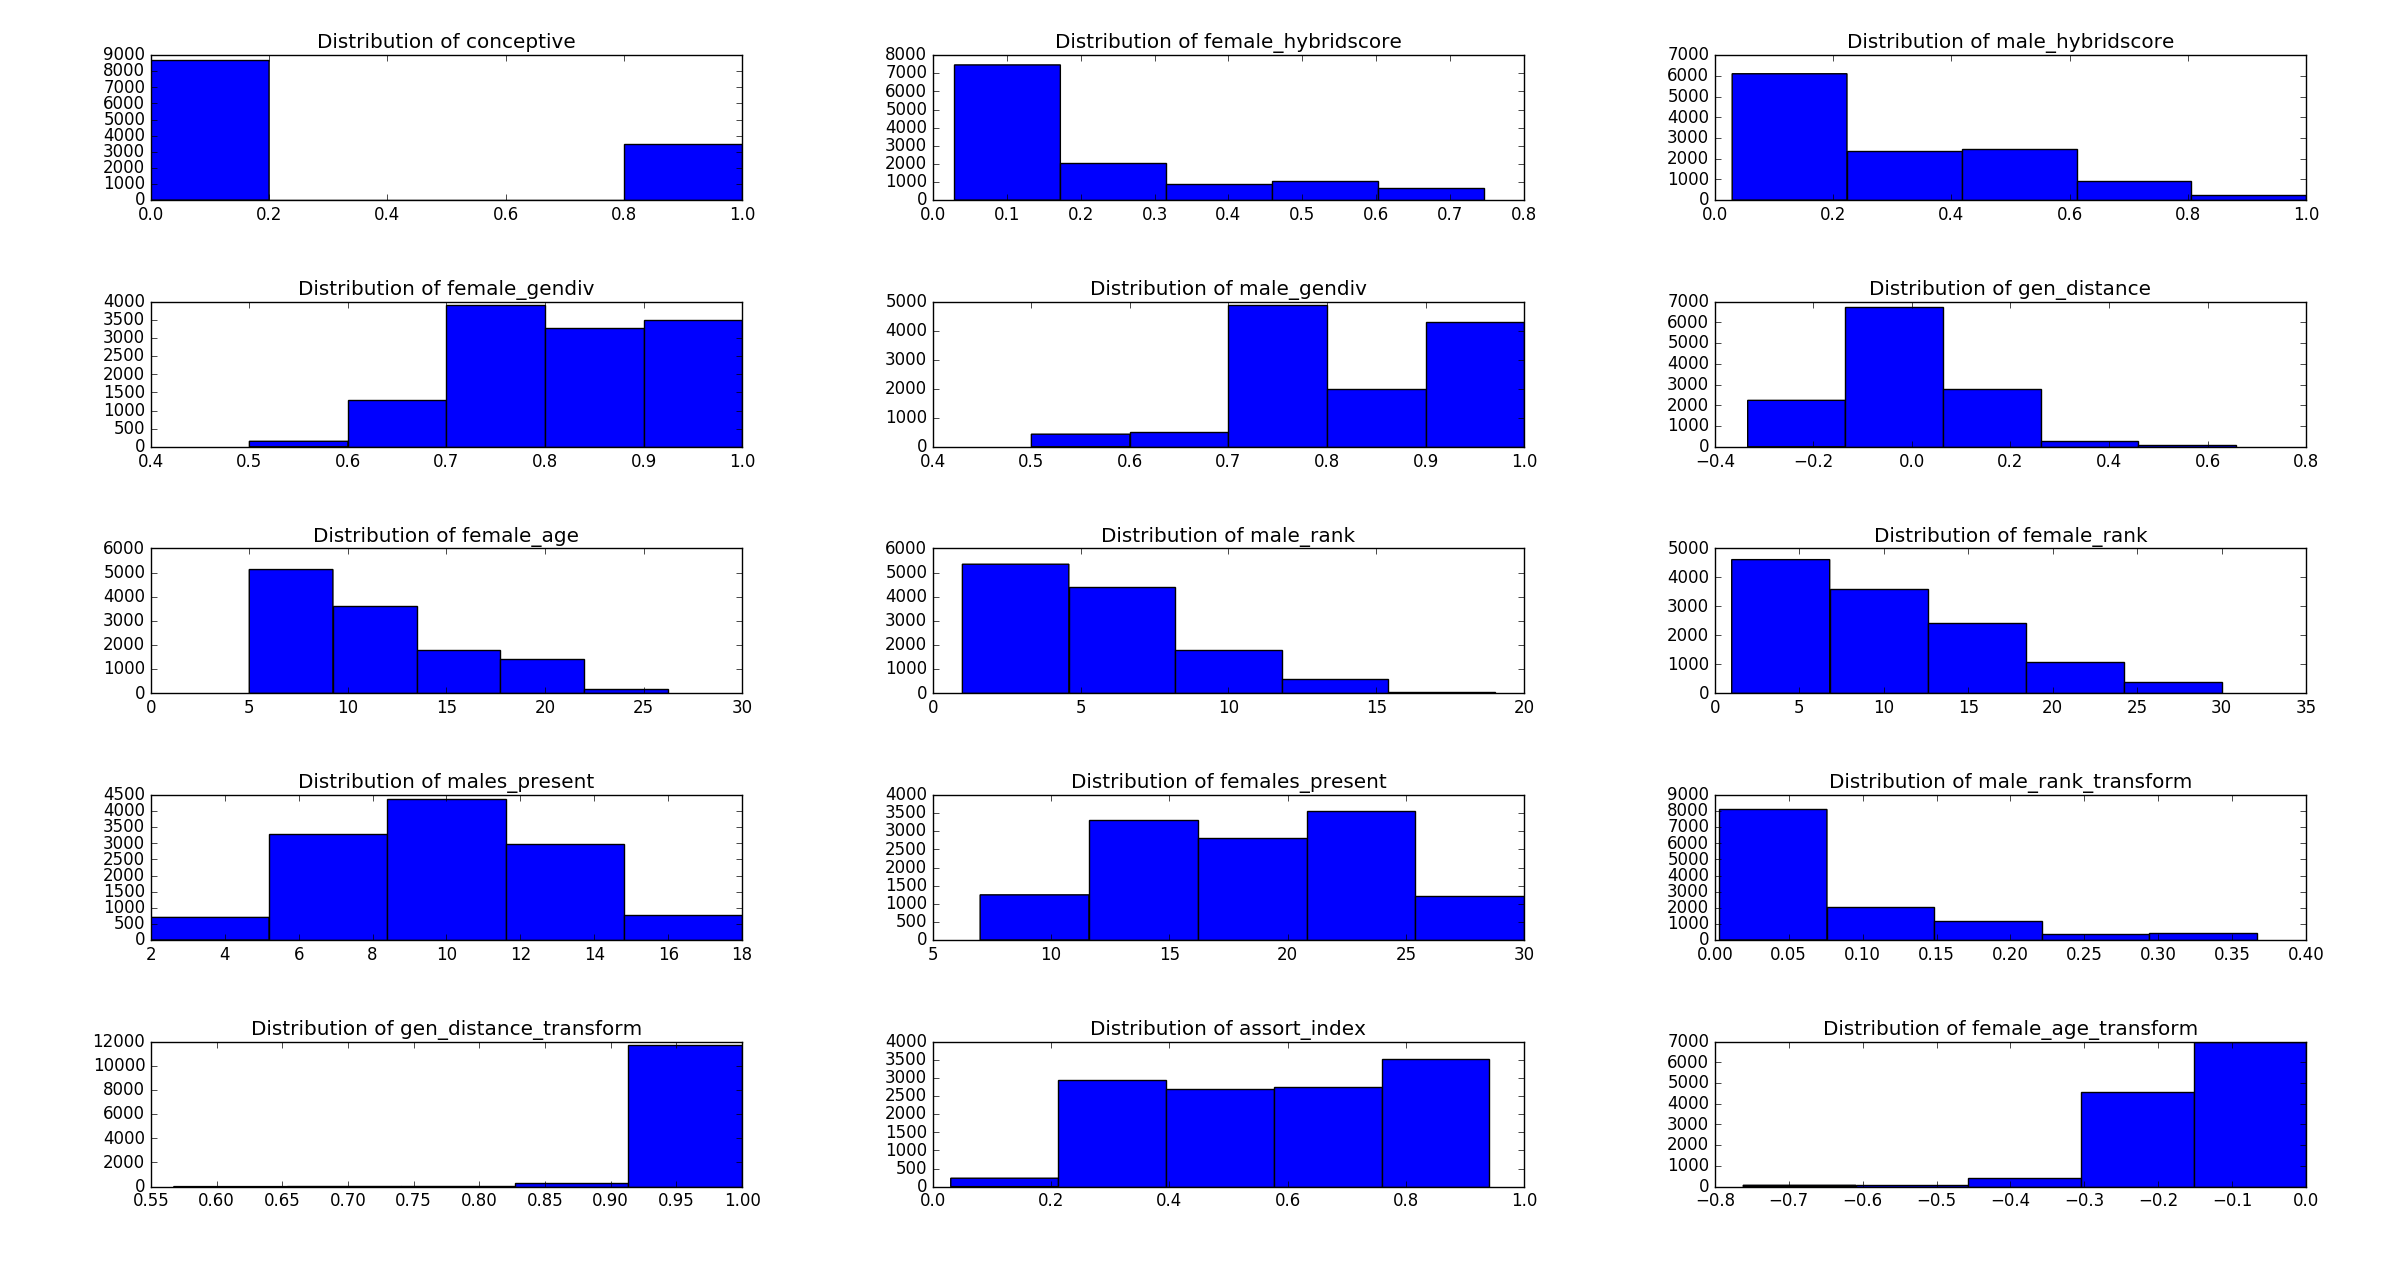
\includegraphics[width=0.5\textwidth]{../figs/all_feats_histogram.png}
  %\caption{Distribution of features}
  %\label{fig:figure_distrib}
%\end{figure}

%\begin{figure}[h]
      %\centering
          %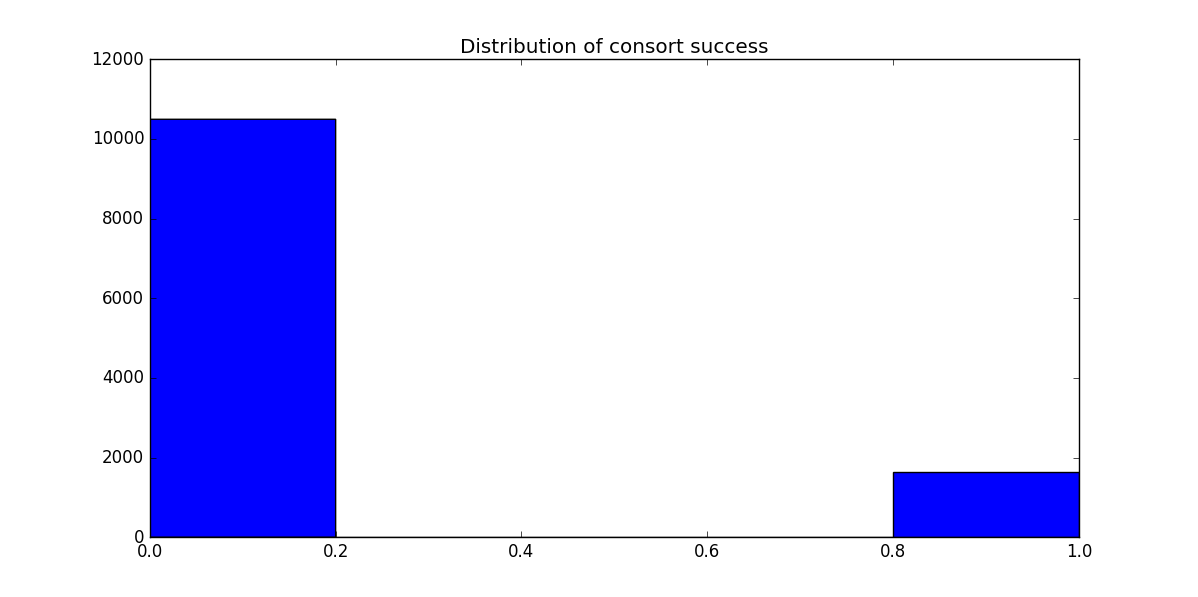
\includegraphics[width=0.5\textwidth]{../figs/consort_distrib.png}
  %\caption{Distribution of consort/non-consort labels}
  %\label{fig:label_distrib}
%\end{figure}
We observe that the labels within the dataset are imbalanced -- there are
approximately 5 times as many pairs which did not consort than those who did.
This imbalance may cause an issue in our classification algorithms. To avoid
this we use the \texttt{weight} for \texttt{scikit-learn}'s classifiers to
automatically assign weights to the classes based on the incidence of labels.\\
% PCA results
\begin{figure}
      \centering
          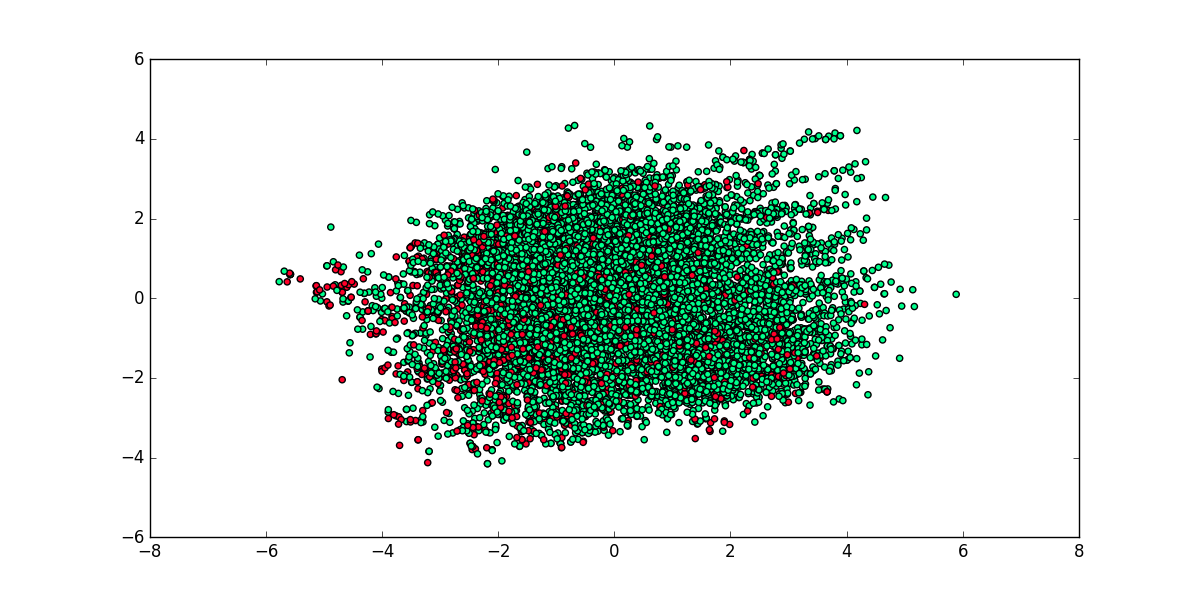
\includegraphics[width=0.5\textwidth]{../figs/consort_non_consort_visualization_pca.png}
  \caption{Reduced-dimensionality PCA visualization of consorting (red) and
  non-consorting pairs (green)}
  \label{fig:pca_vis}
\end{figure}

Using PCA to map higher dimensional dataset to 2 dimensions does not reveal
any lower-dimensional separation between the consorting/non-consorting pairs, as
shown in Figure \ref{fig:pca_vis}.
This indicates that the classification problem may be inherently
high-dimensional. The tSNE manifold mapping indicates this as well.

\subsection{Preprocessing}

We experimented with several preprocessing methods for the dataset. We removed
points that were nearly identical, but had different labels. Additionally, when
training classification models, we normalized the features, based on the mean
and standard deviation of the training set. Because our dataset has an imbalance
between positive and negative labels, we tried augmenting our set by adding in
synthetic positively labelled points which were derived from existing positively
labelled points with some small amount of random noise added to each of the
features. In addition, we considered using PCA whitening, in which the feature
space used is based on the principal components of the dataset in order to
reduce correlation across the features. However, we found that augmentation and
PCA whitening did not improve our results, and so chose not to use these
techniques.

\section{Methods}
\subsection{Materials}

To perform our analysis, we used the \texttt{scikit-learn} python package (\cite{Pegregosa:2011}). Methods
that were not readily available in \texttt{scikit-learn}, such as feature selection, were
implemented independently in python.

\subsection{Classification}
To examine if we can predict consortship, we perform a K-fold validation with 10
folds over several linear and non-linear classifiers, each embedded in a forward
feature selection algorithm framework. In general, for each algorithm, we tuned
the hyper-parameters manually by iteratively running the model with different
parameters and checking the training and testing errors and F1 scores to ensure
that we were not overfitting to the training set.  Additionally, we ensured that
the class weights were balanced, given that the negative (non-consort) labels
outweigh the positive labels (consort) by 5-to-1. When performing K-fold
validation, the data was randomly shuffled so as to avoid positive labels
concentrating in a particular training or test set, biasing the performance.
Moreover, for each algorithm and feature subset we evaluate the error,
precision, recall, F1, and AUC scores as an average on
each of the K-cluster training and test sets. Finally we store the confusion
matrix, obtained by running 75-25 hold-out cross-validation with all the
features and for the models that performed best.
\begin{table}[h]
  \centering
  \begin{tabular}{|l|c|}
    \hline
    Summary Statistic & Description \\
    \hline
    Precision&
    $\frac{\#\ true\ positive}{\#\ true\ positive + \#\ false\ positive}$\\
    \hline
    Recall (F1) Score &
    $\frac{\#\ true\ positive}{\#\ true\ positive + \#\ false\ negative}$\\
    \hline
    Fischer (F1) Score &
    $\frac{2* precision* recall}{{precision}+{recall}}$\\
    \hline
    AUC &
    Area under ROC curve \\
    \hline
  \end{tabular}
  \caption{Description of summary statistics}
  \label{tbl:sum_stats}
\end{table}

 The gaussian SVM tries to optimize: \\
 $$ \min_{w,b,\xi} \frac{1}{2} w^Tw + C \sum_{i=1}^{n} \xi_i$$ $$ s.t. \ \  y_i(w^T\phi(x) + b) >= 1-\xi_i$$ where $\phi(x)$ is the Gaussian feature mapping, (w,b) are the functional margin and $\xi$ is the extent to which misclassified points lie outside the functional margin.
We used a penalty parameter of $C=10$.\\

In addition, we examined boosted decision trees with AdaBoosting and Random
Forests, which are ensemble methods. Both of our ensemble methods use decision
trees as their constituent classifiers. Decision trees define labels based on a
tree of thresholds applied to different features -- they can be considered multi-level decision stumps.\\

AdaBoosting is trained over several iterations. At each iteration, a weak
learner is trained on a weighted dataset, where the weight in iteration $t$ is
given by: $$E_t=\sum_i E[F_{t-1}(x_i) + \alpha_t h(x_i)]$$ \\
$$\epsilon_m = \frac{\sum_{y_i \ne k_m(x_i)} w_i^m}{\sum_i w_i^m}$$
$$\alpha_t=\frac{1}{2}ln(\frac{1-\epsilon_t}{1+\epsilon_t})$$ where $E_t$ is the training error, $F_{t-1}$ is the current boosted classifier, h(x) is the output of each new weak learner and $\alpha_t$ is the weight of the new learner. To calculate $\alpha_t$, the error rate $\epsilon_m$ of the new weak classifier needs to be computed first.
We use 8 weak learners in AdaBoosting, where each learner is a decision tree with a maximum depth of 4.\\

Random forests train several decision trees on a random subset of the features.
Classifications are then determined by taking a majority vote across the trees.
We use random forests of 13 decision trees with maximum depth 4 and with the
maximum number of features set to the square root of the total number of
features.

% TODO: figure out whether to include subsequent paragraph
We experimented with several additional classifiers with regularization, including logistic
regression, linear and polynomial SVM, and Naive Bayes. However, these
classifiers had very poor performance and we have excluded their discussion due
to space constraints.

\subsection{Graphical Approach}

\subsubsection*{Classification}
%------------------------------------------------
Another approach to predicting consortship is to use the interactions as edges
and the baboons as nodes. Due to only heterosexual interactions, the resulting
graph is bipartite. This transforms the classification task to an edge
prediction task. Most previous work on this has been on just predicting whether
or not edges exist, not predicting the label of the edge. We adapted current
methods to predict the label of an edge rather than its existence.\\ 

\cite{Macskassy:2007} use a simple method that computes the similarities of the
attributes of nodes to determine the weight of latent edges between nodes. Their method is used to determine latent edges in text documents. Because most of the features are not inherent to the baboons, but are
depdendent on the interaction between individuals, we adapt this method to look
at the similarity between the proposed edge and already existing edges between
those two nodes. More formally, if there is some set of nodes $V$ and some set
of edges $E$ where each edge $e_i$ has some associated features $f_i$ and some
associated label $l_i\in \{0,1\}$ then to determine the label of a new edge
$e_n$ between nodes $u$ and $v$ we would compute $argmax_{label \in \{0,1\}}
\frac{\sum_{e_i \in E}1\{l_i=label\}\cdot|e-e_n|_2}{\sum_{e_i \in
E}1\{l_i=label\}}$. This is essentially the same as KNN where $K=1$. %We also tried the same model except for only looking at edges where one of the endpoints was $u$ or $v$, formally: $argmax_{label \in \{0,1\}} \frac{\sum_{e_i \in E:u \in e_i \; or\; v \in e_i}1\{l_i=label\}\cdot|e-e_n|_2}{\sum_{e_i \in E:u \in e_i \; or\; v \in e_i}1\{l_i=label\}}$. However this performed much worse

\subsubsection*{Additional Features}

In order to try to capture latent features that are not present in the dataset,
such as the popularity or charisma of individuals, we compute PageRank and HITS scores of individual baboons based on their their successful consortships in the
training set, where nodes are the male and female baboons and edges exist for
successful consortships.  For both PageRank and HITS we treated baboons as vertices, and consorts between baboons as undirected edges between them, and we ignored non-consorts. For PageRank we use the standard algorithm by \cite{Domingos:2002} then create an adjacency matrix $M$ and then find the eigenvector associated with the principle eigenvalue of $A$ where $A=\beta M+(1-\beta)\cdot[\frac{1}{n}]_{nxn}$ where $\beta$ is used to essentially smooth the distribution. We used $\beta=.1$. The PageRank score of each baboon is the value of the eigenvector at its corresponding index from the adjacency matrix. For HITS we use the standard algorithm by \cite{Kleinberg:1998} compute the hub and authority score by initializing each female's hub score to 1 and each male's authority score to 1. We then update the hub score of each female to be the sum of the authority score of all males she is connected to divided by that male's degree. We similarly update the authority of each males score. We then normalize the hub and authority scores and then repeat 1000 times. At the end we assign the authority score as their HITS score, and the hubs score of the females as their HITS score.
We evaluated the effectiveness of adding these features to our classifiers as well
as just classifying based on these features alone.

\subsection{Clustering}
% kmeans on non-consort pairs, examined centroids, used PCA to visualize

We ran the k-means algorithm on the consorting and
non-consorting pairs. k-means clusters the data by first randomly guessing
centroids of the clusters. Then until convergence is reached the following steps
are repeated: for each data
point i is assigned to a group j, $c^{(i)}$, where
$c^{(i)}:=\arg\min_{j}||x^{(i)}-\mu_j||^2$, where $\mu_j$ is the coordinate of
the of the estimated centroid of the group. Then for each $j$,
$\mu_j:=\frac{\sum_{i=1}^m1\{c^{(i)}=j\}x^{(i)}}{\sum_{i=1}^m{c^{(i)}=j}}$.
To visualize the clusters, we then used dimensionality
reduction techniques such as PCA and the t-SNE manifold tool. We chose to use 5
clusters based visualizing the clustering results and choosing the value that
gave us the cleanest separation.

\section{Results and Discussion}
\subsection{Classification}
% confusion matrix

\begin{figure}[h]
      \centering
      \begin{tabular}{| l |c |c |c |c|}
        \hline
        & \multicolumn{2}{ |c| }{Error} & \multicolumn{2}{ |c| }{F1} \\
        \hline
        & Train  & Test & Train  & Test \\
        \hline
        Gaussian SVM &  0.286 & 0.339 & 0.438 & 0.363 \\
        AdaBoosting & 0.329 & 0.353 & 0.377 & 0.339 \\
        Random Forest & 0.342 & 0.340 & 0.325 & 0.343 \\
        Edge Prediction & 0.410 & 0.464 & 0.273  & 0.259 \\
        \hline
      \end{tabular}
  \caption{Summary of test/train errors and F1 scores}
  \label{fig:rbf_svm_vis}
\end{figure}

Running forward feature selection shows that, for all the classifiers
considered, the best performance in terms of the designated metrics is achieved
with a combination of biological and social features. Additionally, we found that
the derived features added by the original researchers did not contribute
significantly to improving the predictive power of our classifiers.\\

\begin{figure}[h]
      \centering
      Gaussian SVM
      \begin{tabular}{|l|c|c|c|c|}
        \hline
        Name & Type & Error & F1 & AUC \\
        \hline
        female\_hybridscore  & BG  & 0.50  & 0.25 & 0.55\\
        male\_hybridscore  & BG  & 0.48 & 0.25 & 0.56\\
        female\_gendiversity & BG  & 0.46 & 0.27 & 0.58\\
        male\_gendiversity & BG  & 0.42 & 0.29 & 0.61\\
        gen\_distance & BG  & 0.39 & 0.31 & 0.63\\
        female\_age &  BG  & 0.35 & 0.35  & 0.67\\
        male\_rank & S & 0.35 & 0.35 & 0.67\\
        female\_rank & S & 0.32 & 0.36  & 0.67\\
        \hline
      \end{tabular}
      AdaBoosted Decision Trees
      \begin{tabular}{|l|c|c|c|c|c|}
        \hline
        Name & Type & Error & Fischer & AUC \\
        \hline
        male\_rank & S & 0.33 & 0.31 & 0.62 \\
        male\_hybridscore & DP & 0.37 & 0.32 & 0.64 \\
        inbreeding\_avoid\_index & DP & 0.36 & 0.32 & 0.64 \\
        gen\_distance & BG & 0.37 & 0.33 & 0.64 \\
        males\_present & S & 0.36 & 0.34 & 0.65 \\
        \hline
      \end{tabular}
      Random Forest
      \begin{tabular}{|l|c|c|c|c|c|}
        \hline
        Name & Type & Error & Fischer & AUC \\
        \hline
        male\_rank\_transform & DS & 0.36 & 0.31 & 0.62 \\
        male\_hybrid\_score & BG & 0.32 & 0.31917 & 0.63 \\
        males\_present & S & 0.34 & 0.32 & 0.63 \\
        females\_present & S & 0.33 & 0.33 & 0.64 \\
        \hline
      \end{tabular}
  \caption{Forward feature selection for classifiers showing features selected
    at each step. Metrics reported are averages on the test sets averaged over a
    10-fold cross validation.  Feature types are denoted as follows: BG -
    biological/genetic, S: Social, DP: Derived Pairwise}
  \label{tbl:feat_selection}
\end{figure}

Moreover when breaking down the performance of each classifier, the top pick is
gaussian SVM, followed by AdaBoosting, and Random Forests. However, we note
that AdaBoosting and Random Forests are more parsimonious and require fewer
features than the SVM. 
\\

Since the labels in our dataset are imbalanced, low error rates may mask poor
performance on positive labels. Thus we focused on examining the Fischer and AUC
scores, which capture the performance of the model both in terms of false positives and false negatives. On the whole, the Fischer and AUC scores are comparable
across the models that we examined. Based on the relatively low difference
between the training and testing metrics, we do not believe that we are
overfitting to our training data, which indicates that we applied sufficient
regularization to our models.
\\

\begin{table}[h]
  \centering
  \begin{tabular}{| l |l |c |c|}
    \hline
    & & \multicolumn{2}{ |c| }{Predicted} \\
    \hline
    & & Consort & Non-Consort \\
    \hline
    \parbox[t]{2mm}{\multirow{2}{*}{\rotatebox[origin=c]{90}{True}}} & Consort & 0.69 & 0.31  \\
                                                                     & Non-Consort & 0.36 & 0.64 \\
    \hline
  \end{tabular}
  \caption{Gaussian SVM normalized confusion matrix in 75-25 cross-validation.}
  \label{tbl:cm_rbf_vis}
\end{table}
\begin{table}[h]
  \centering
  \begin{tabular}{| l |l |c |c|}
    \hline
    & & \multicolumn{2}{ |c| }{Predicted} \\
    \hline
    & & Consort & Non-Consort \\
    \hline
    \parbox[t]{2mm}{\multirow{2}{*}{\rotatebox[origin=c]{90}{True}}} & Consort & 0.65 & 0.35  \\
                                                                     & Non-Consort & 0.35 & 0.65 \\
    \hline
  \end{tabular}
  \caption{AdaBoosting normalized confusion matrix in 75-25 cross-validation.}
  \label{tbl:cm_lin_vis}
\end{table}
\begin{table}[h]
  \centering
  \begin{tabular}{| l |l |c |c|}
    \hline
    & & \multicolumn{2}{ |c| }{Predicted} \\
    \hline
    & & Consort & Non-Consort \\
    \hline
    \parbox[t]{2mm}{\multirow{2}{*}{\rotatebox[origin=c]{90}{True}}} & Consort & 0.66 & 0.34  \\
                                                                     & Non-Consort & 0.36 & 0.64 \\
    \hline
  \end{tabular}
  \caption{Random Forest normalized confusion matrix in 75-25 cross-validation}
  \label{tbl:cm_lin_vis}
\end{table}

\begin{table}[h]
  \centering
  \begin{tabular}{| l |l |c |c|}
    \hline
    & & \multicolumn{2}{ |c| }{Predicted} \\
    \hline
    & & Consort & Non-Consort \\
    \hline
    \parbox[t]{2mm}{\multirow{2}{*}{\rotatebox[origin=c]{90}{True}}} & Consort & 0.531 & 0.469  \\
                                                                     & Non-Consort & 0.434 & 0.566 \\ %F1 score of .259
    \hline
  \end{tabular}
  \caption{Edge Prediction normalized confusion matrix in 75-25 cross-validation}
  \label{edge_pred}
\end{table}
\begin{table}[h]
  \centering
  \begin{tabular}{| l |l |c |c|}
    \hline
    & & \multicolumn{2}{ |c| }{Predicted} \\
    \hline
    & & Consort & Non-Consort \\
    \hline
    \parbox[t]{2mm}{\multirow{2}{*}{\rotatebox[origin=c]{90}{True}}} & Consort & 0.54 & 0.46  \\
                                                                     & Non-Consort & 0.35 & 0.65 \\
    \hline
  \end{tabular}
  \caption{AdaBoosting normalized confusion matrix using just derived graphical features.}
  \label{tbl:page_rank_hits_confusion}
\end{table}


% TODO: additional discussion of confusion matrices

\subsection{Graphical Approach}
\subsubsection*{Classification}

%------------------------------------------------
The edge prediction method in Table \ref{edge_pred} does quite poorly compared to SVM and other approaches, but this is not surprising since it is a very simple classifier. We tried adding HITS and PageRank scores to the provided features, however there was little improvement in any of the models. However, when using HITS and PageRank as the only features (Table \ref{tbl:page_rank_hits_confusion}) the performance is suprisingly good especially given that there is no information being used other than what baboons consorted in the past. %TODO ADD IN CONFUSION MATRIX WITH LABEL HITS_PageRank

\subsection{Clustering}
\begin{figure}[h]
      \centering
          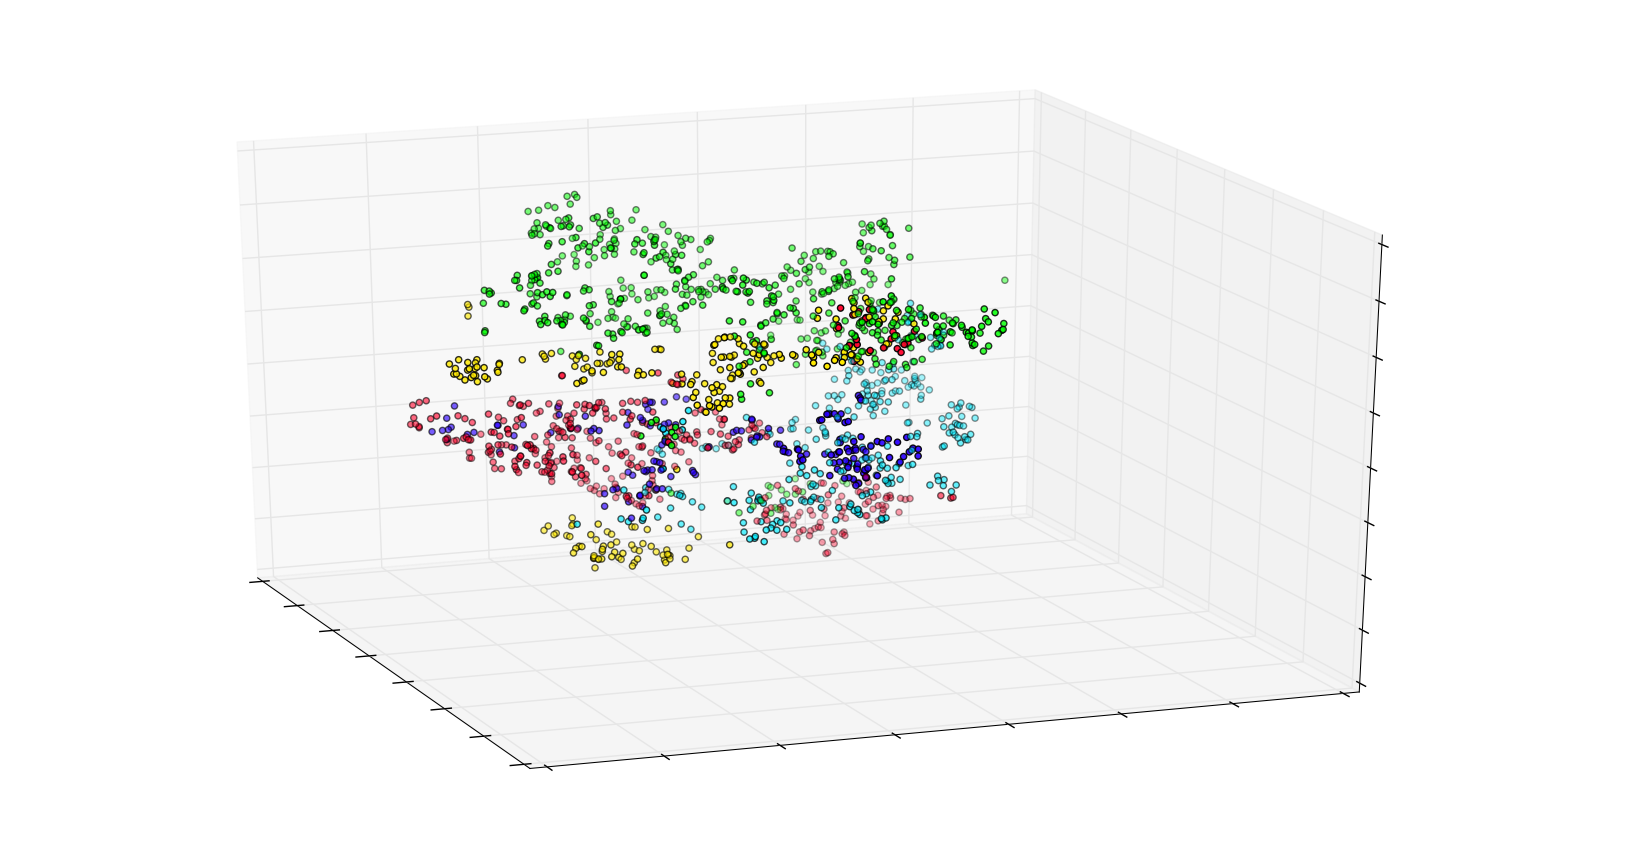
\includegraphics[width=0.5\textwidth]{../figs/consort_kmeans_5_3d_tsne.png}
  \caption{t-SNE visualization of K-Means with 5 clusters applied on consorting
  pairs. Red: High Male Rank, Cyan: Old Females, Green: Low number of males
present, Violet: Low number of females present, Yellow: High number of males
present.}
  \label{fig:consort_clustering_vis}
\end{figure}

By visualizing clustering results, we found that the clusters for non-consorting
pairs were not cleanly separated -- it was difficult to cluster non-consorting
pairs. On the other hand, the lower-dimensional visualization of consorting
clusters  (Figure \ref{fig:consort_clustering_vis}) shows cleaner separation for
the consorting pairs than for the non-consorting pairs. This indicates that it
may not be possible to group non-consortship, there are clusters of consortships
that share common features.


\section{Conclusion and Future Work}

We found that both social and genetic factors are useful in predicting
consortship, which agrees with the results in \cite{Tung:2012}. However, we
found that the additional derived features added by in the original study did
not significantly improve our classification results. Additionally, we found
that clusters exist within consortships, implying that there are different types
of consortships.\\
The somewhat comparable performance of HITS and PageRank without any other features is interesting because this means that researchers would only have to gather data on who mated with whom and would still be able to get similar results without having to do genetic tests, figure out how old the baboons were, or any other time and resource intensive data gathering. 
Generally, we found similar classification results with Gaussian SVM,
AdaBoosting, and Random Forests, with the Gaussian SVM at a slight edge over the
others. Generally, all of our models sufferred from high rates of false
negatives, which we believe to be partially attributable to the imbalance of
positive and negative labels. Additionally, there may be features that impact
consortship that are not captured by the dataset. We expect that modeling these
latent features using graphical approaches to be a valuable area of
investigation. While the graph-based features we added only helped marginally,
algorithms that are specialized to work on bipartite graphs may provide more
significant improvement. We do not expect that the classification problem to be
solved completely, as there may be many factors in the formation of
relationships between intelligent, social mammals that we cannot capture.
\\

If our team had more time to work on this problem, we would explore the
development of additional graphical methods to supplement our features.
Additionally, we would try to obtain a dataset that has a larger set of features
(such as additional phenotypes or genotypic markers), or more datapoints.
Finally, the dataset that we used was constructed by tracking different packs of
baboons. It may be interesting to examine whether modeling each pack separately
would improve our results, and whether different social factors have different
explanatory power across the groups.
\\

%----------------------------------------------------------------------------------------
%	REFERENCE LIST
%----------------------------------------------------------------------------------------

\begin{thebibliography}{99} % Bibliography - this is intentionally simple in this template

\bibitem [Domingos, 2002]{Domingos:2002} 
P. Domingos, M. Richardson (2002) 
\newblock
 The Intelligent Surfer: Probabilistic Combination of Link and Content Information in PageRank
\newblock{\em Proceedings NIPS}, 2002

\bibitem [Kleinberg, 1998]{Kleinberg:1998} 
J. Kleinberg
\newblock
Authoritative sources in a hyperlinked environment
\newblock{\em Proceedings 9th ACM-SIAM Symposium on Discrete Algorithms}, 1998

\bibitem [Macskassy, 2007]{Macskassy:2007} 
Sofus A. Macskassy (2007) 
\newblock
Improving learning in networked data by combining explicit and mined links
\newblock{\em Proceedings of the 22nd national conference on Artificial intelligence}, July 22-26, 2007, p.590-595
 
\bibitem[Pedregosa, et al. 2011]{Pegregosa:2011}
  Pedregosa, \em{et al.} (2011)
  \newblock
  Scikit-learn: Machine Learning in Python
  \newblock{JMLR}, 2011 12, 2825--2830.

\bibitem[Tung et al., 2012]{Tung:2012}
  Jenny Tung, Marie J. E. Charpentier, Sayan Mukherjee, Jeanne Altmann, and Susan C. Alberts (2012)
\newblock 
  Genetic Effects on Mating Success and Partner Choice in a Social Mammal.
\newblock {\em The American Naturalist}, 2012 180:1, 113--129.

\end{thebibliography}

%----------------------------------------------------------------------------------------

\end{document}
